\documentclass{acmsiggraph}
\usepackage{mathptmx}
\usepackage{graphicx}
\usepackage{epsfig}
\usepackage{amsmath,amscd,amssymb}
\usepackage{hyperref}

\newtheorem{theorem}{Theorem}[section]
\newtheorem{proposition}[theorem]{Proposition}
\newtheorem{definition}[theorem]{Definition}
\newtheorem{lemma}[theorem]{Lemma}
\newtheorem{corollary}[theorem]{Corollary}
\newtheorem{remark}[theorem]{Remark}

\usepackage{parskip}

\onlineid{papers\_0142}

\acmformat{cameraready}

\title{CS 4/553 Term Project: Visualizing the Loss Landscape of Neural Nets}

\author{Charles Ison\thanks{\small\texttt{e-mail: \{isonc|morgamat\}@eecs.oregonstate.edu}}\\ Oregon State University
\and Matthew Morgan$^{\ast}$ \\
Oregon State University}

\keywords{loss landscape, scalar field topology, neural networks, gradient descent}

\begin{document}

\teaser{
	%\centerline{\epsfig{file=images/teaser.eps,angle=0,width=\textwidth}}
	$\begin{array}{@{\hspace{-0.00in}}c@{\hspace{0.10in}}c@{\hspace{0.10in}}c@{\hspace{0.05in}}c}
			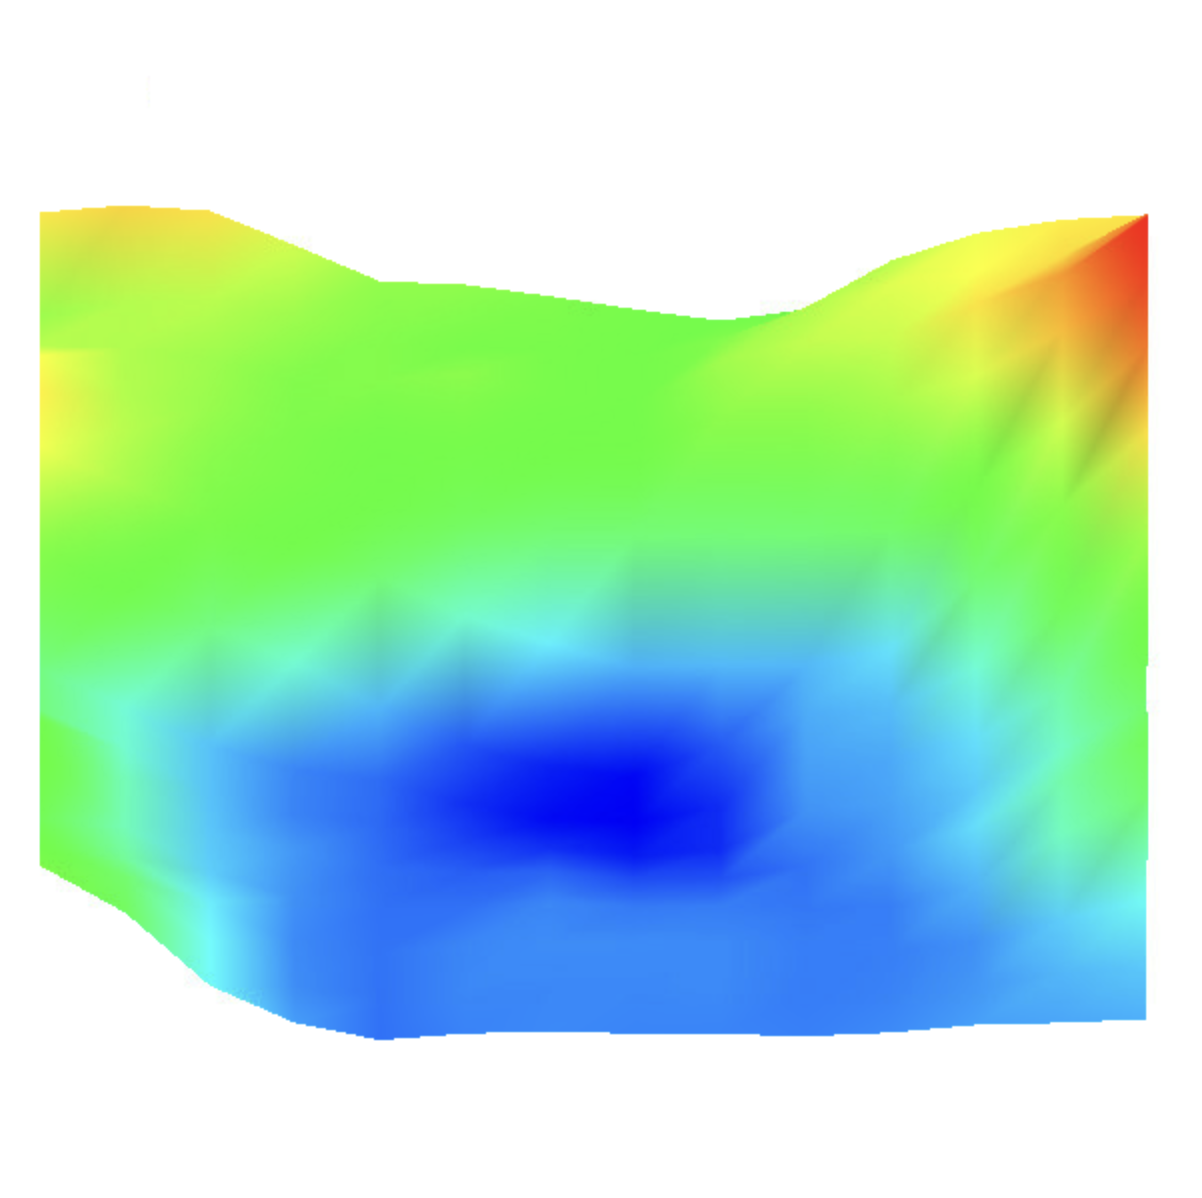
\includegraphics[width=2.50in]{images/resnet_normalized_color.png}
			&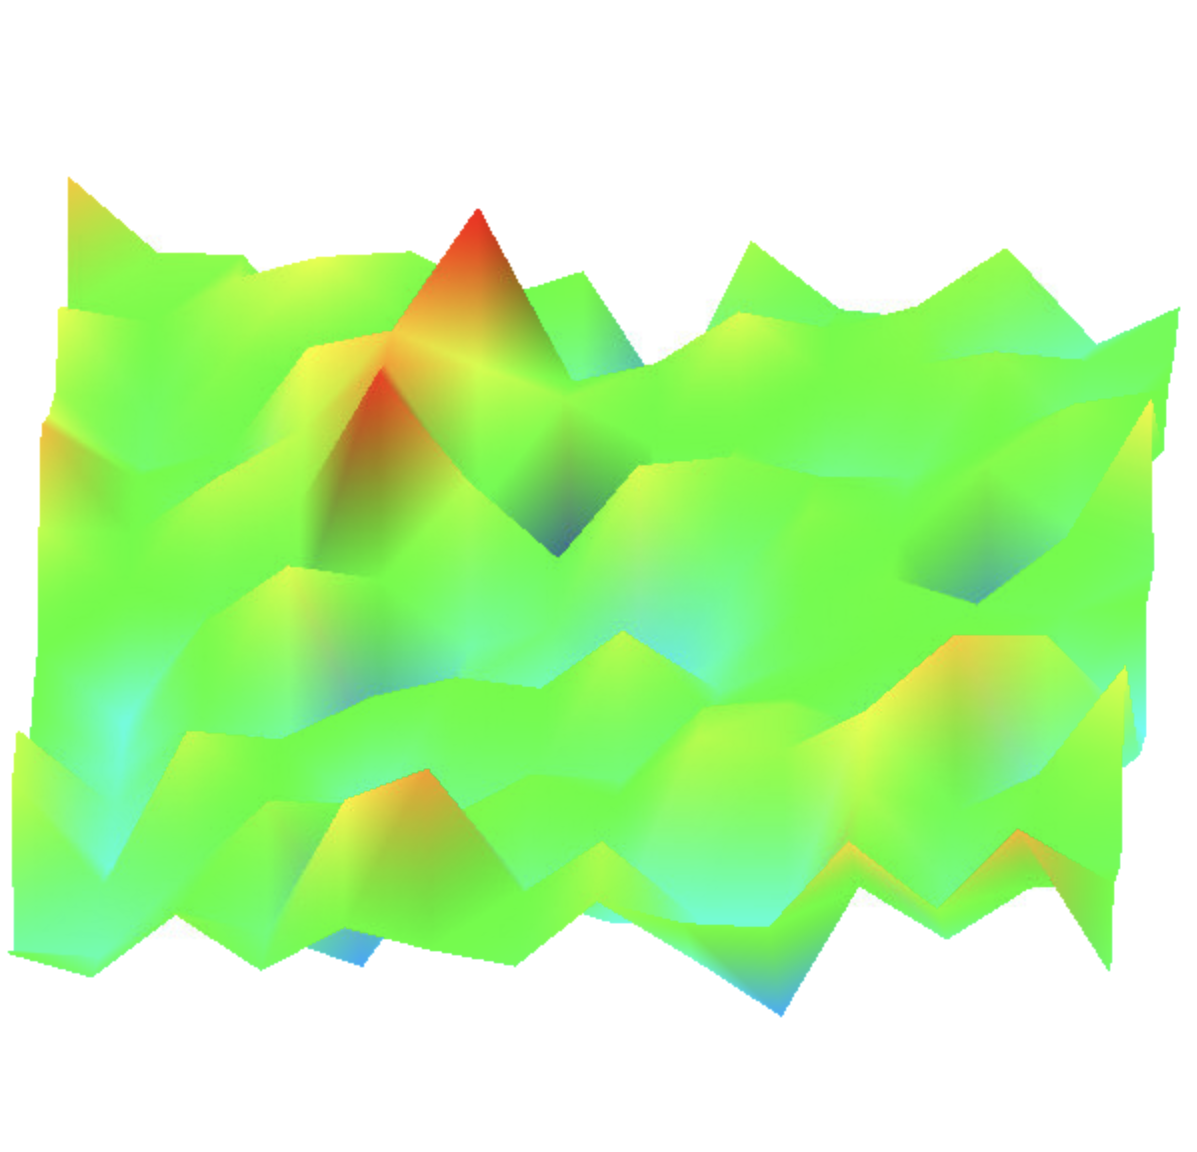
\includegraphics[width=2.50in]{images/vgg-normalized-color.png}
			\\
			(a)  &  (b)
		\end{array}$
	\caption{The loss landscapes of two different models trained on the same dataset for the same number of epochs: 
	(a) ResNet50, and (b) VGG11. } \label{fig:teaser} }

\maketitle
\keywordlist


\begin{abstract}

	\copyrightspace
	
	TODO:
	Designing rotational symmetries on surfaces is a necessary task for
	a wide variety of graphics applications, such as surface
	parameterization and remeshing, painterly rendering and pen-and-ink
	sketching, and texture synthesis. In these applications, the {\em
	topology} of a rotational symmetry field such as {\em singularities}
	and {\em separatrices} can have a direct impact on the quality of
	the results. In this paper, we present a design system that provides
	control over the topology of rotational symmetry fields on surfaces.
	
	As the foundation of our system, we provide comprehensive analysis
	for rotational symmetry fields on surfaces and present efficient
	algorithms to identify singularities and separatrices. We also
	describe design operations that allow a rotational symmetry field to
	be created and modified in an intuitive fashion by using the idea of
	basis fields and relaxation. In particular, we provide control over
	the topology of a rotational symmetry field by allowing the user to
	remove singularities from the field or to move them to more
	desirable locations.
	
	At the core of our analysis and design implementations is the
	observation that $N$-way rotational symmetries can be described by
	symmetric $N$-th order tensors, which allows an efficient
	vector-based representation that not only supports coherent
	definitions of arithmetic operations on rotational symmetries but
	also enables many analysis and design operations for vector fields
	to be adapted to rotational symmetry fields.
	
	To demonstrate the effectiveness of our approach, we apply our
	design system to pen-and-ink sketching and geometry remeshing.
	
\end{abstract}

\begin{CRcatlist}
	\CRcat{I.3.5}{Computer Graphics}{Computational Geometry and
	Object Modeling}{Geometric algorithms, languages, and systems};
\end{CRcatlist}

%% The ``\keywordlist'' command prints out the keywords.
\keywordlist


\section{Introduction}
\label{sec:intro}

Neural networks are machine learning models constructed from interconnected nodes. 
Backpropagation through gradient descent is one commonly used algorithm for training neural networks.
By visualizing neural network loss functions as scalar fields, can we better understand the impact of various network architectures on the model’s trainability.


In this project, we implement the paper "Visualizing the Loss Landscape of Neural Nets" (\url{https://arxiv.org/pdf/1712.09913.pdf}) for Option 2 (implementing a published research paper). 
By mapping the loss of a neural network across two dimensions, we create scalar field visualizations of various neural network architectures that the paper authors call “Loss Landscapes.” 
In these visualizations, the loss function’s results serve as the scalar value and a two dimensional reduction of the model’s weights serves the directional elements of the field. 
The specific loss functions used in the original paper are cross entropy (\url{https://pytorch.org/docs/stable/generated/torch.nn.CrossEntropyLoss.html}) and mean squared error (\url{https://pytorch.org/docs/stable/generated/torch.nn.MSELoss.html}).
The dimensionality reduction is done using two different approaches: principal component analysis and random vector selection. 
For the later approach, two random vectors within the input space are created by sampling a random Gaussian distribution. 
These vectors are used as the two dimensions of the scalar field input. 
The resulting loss landscapes generated can then provide insights into how certain architectural decisions can improve or worsen a network's trainability.


\section{Previous Work}
\label{sec:previous_work}

There have been numerous studies on the ability to optimize neural loss functions in order to improve training time and model performance. 
Less work has been conducted on visualizing the losses though to gain intuition about how certain architectural decisions impact the loss field's convexity. 
However, one paper by ~\cite{hochreiter1997flat} defined “flatness” as the size of the connected region around the minimum where the training loss remains low which is visualized by this work. Since the paper was released in 2018, numerous other works have cited it. However, many of the citations are not from works attempting to advance the visualizations, but rather to learn from the visualizations and develop more generalizable and accurate models. The visualizations have come in handy for researchers studying reinforcement learning models such as \cite{actor2020} and \cite{plaat2022deep}.

There are some recent works which produce new visualizations of loss functions. One such by ~\cite{pmlr-v137-huang20a}, "Understanding Generalization Through Visualizations", use
visualization methods to give intuitions about why certain architectures generalize better than others. They first visualize loss as a scalar field with height and color representing the output. But they also use a colored dot plot and a "Swissroll decision boundary" to show the difference in models that perform well versus models that perform poorly at generalizing.

An interesting extension of this work by ~\cite{linse2022walk} visualizes large neural networks in virtual reality. The approach allows for high interactivity, but requires a virtual reality headset and powerful computer to render.


\section{Background}
\label{sec:intro}

TODO:
Magnam nulla non possimus est error aliquam non iste. Hic praesentium perspiciatis numquam. Necessitatibus aut mollitia porro quod. Libero voluptatum illo exercitationem incidunt voluptate. Vero ut sapiente quia nisi possimus non. Consequuntur molestiae voluptas eum illo ut quo qui.
Et quod dolore maxime. Quo omnis ut a iure ut facere. Asperiores et explicabo aliquid omnis ratione laborum libero. Aperiam fuga facilis soluta non suscipit.
Saepe velit ut iusto dolorum beatae quae expedita. Facere quia aut architecto velit quibusdam iste. Explicabo a provident debitis. Quia dolore numquam qui laboriosam consectetur necessitatibus.
Quisquam officiis placeat vitae necessitatibus aut. Iure libero quae nostrum expedita quis voluptates harum. Delectus natus amet nihil voluptatem corporis maxime. Necessitatibus natus aut tempore aut et.
Eos facilis aut id commodi quis id maiores. Labore distinctio nobis deserunt perferendis perferendis perferendis laborum temporibus. Dignissimos nostrum laudantium enim unde numquam temporibus ipsa. Qui ut officia enim est deserunt.


\section{Results}
\label{sec:intro}

TODO:
Magnam nulla non possimus est error aliquam non iste. Hic praesentium perspiciatis numquam. Necessitatibus aut mollitia porro quod. Libero voluptatum illo exercitationem incidunt voluptate. Vero ut sapiente quia nisi possimus non. Consequuntur molestiae voluptas eum illo ut quo qui.
Et quod dolore maxime. Quo omnis ut a iure ut facere. Asperiores et explicabo aliquid omnis ratione laborum libero. Aperiam fuga facilis soluta non suscipit.
Saepe velit ut iusto dolorum beatae quae expedita. Facere quia aut architecto velit quibusdam iste. Explicabo a provident debitis. Quia dolore numquam qui laboriosam consectetur necessitatibus.
Quisquam officiis placeat vitae necessitatibus aut. Iure libero quae nostrum expedita quis voluptates harum. Delectus natus amet nihil voluptatem corporis maxime. Necessitatibus natus aut tempore aut et.
Eos facilis aut id commodi quis id maiores. Labore distinctio nobis deserunt perferendis perferendis perferendis laborum temporibus. Dignissimos nostrum laudantium enim unde numquam temporibus ipsa. Qui ut officia enim est deserunt.


\section{Evaluation}
\label{sec:intro}

TODO:
Magnam nulla non possimus est error aliquam non iste. Hic praesentium perspiciatis numquam. Necessitatibus aut mollitia porro quod. Libero voluptatum illo exercitationem incidunt voluptate. Vero ut sapiente quia nisi possimus non. Consequuntur molestiae voluptas eum illo ut quo qui.
Et quod dolore maxime. Quo omnis ut a iure ut facere. Asperiores et explicabo aliquid omnis ratione laborum libero. Aperiam fuga facilis soluta non suscipit.
Saepe velit ut iusto dolorum beatae quae expedita. Facere quia aut architecto velit quibusdam iste. Explicabo a provident debitis. Quia dolore numquam qui laboriosam consectetur necessitatibus.
Quisquam officiis placeat vitae necessitatibus aut. Iure libero quae nostrum expedita quis voluptates harum. Delectus natus amet nihil voluptatem corporis maxime. Necessitatibus natus aut tempore aut et.
Eos facilis aut id commodi quis id maiores. Labore distinctio nobis deserunt perferendis perferendis perferendis laborum temporibus. Dignissimos nostrum laudantium enim unde numquam temporibus ipsa. Qui ut officia enim est deserunt.


\section{Division of Tasks}
\label{sec:intro}

Charles took responsibility for creating and training the ResNet and VGG models on CIFAR-10 dataset.
He then implemented the dimensionality reduction techniques of principal component analysis and normalized random direction iteration.
Next, by iteratively manipulate the models weights during training and testing, Charles constructed the loss landscape data as tensors from the PyTorch models.
Matthew took responsibility for writing the code to export the loss landscape data from the PyTorch models to PLY files which could be visualized in OpenGL.
Once in OpenGL, Matthew applied the techniques of mapping the landscape to color, visualizing the loss as height, and drawing contour lines across the scalar field.
Additionally, Matthew took data from the model's training iterations and plotted the gradient descent of the model as a curve on the scalar field.
Last, he compared and contrasted the different techniques to find the optimal combinations and discussed how they might be interpreted.
Charles also contributed to the OpenGL visualizations by extracting and showing the critical points, as well as evaluating their correctness.



\section{Conclusions}
\label{sec:intro}

TODO:
Magnam nulla non possimus est error aliquam non iste. Hic praesentium perspiciatis numquam. Necessitatibus aut mollitia porro quod. Libero voluptatum illo exercitationem incidunt voluptate. Vero ut sapiente quia nisi possimus non. Consequuntur molestiae voluptas eum illo ut quo qui.
Et quod dolore maxime. Quo omnis ut a iure ut facere. Asperiores et explicabo aliquid omnis ratione laborum libero. Aperiam fuga facilis soluta non suscipit.
Saepe velit ut iusto dolorum beatae quae expedita. Facere quia aut architecto velit quibusdam iste. Explicabo a provident debitis. Quia dolore numquam qui laboriosam consectetur necessitatibus.
Quisquam officiis placeat vitae necessitatibus aut. Iure libero quae nostrum expedita quis voluptates harum. Delectus natus amet nihil voluptatem corporis maxime. Necessitatibus natus aut tempore aut et.
Eos facilis aut id commodi quis id maiores. Labore distinctio nobis deserunt perferendis perferendis perferendis laborum temporibus. Dignissimos nostrum laudantium enim unde numquam temporibus ipsa. Qui ut officia enim est deserunt.


\begin{figure}[t]
	\begin{center}
		$\begin{array}{@{\hspace{-0.00in}}c@{\hspace{0.05in}}c}
				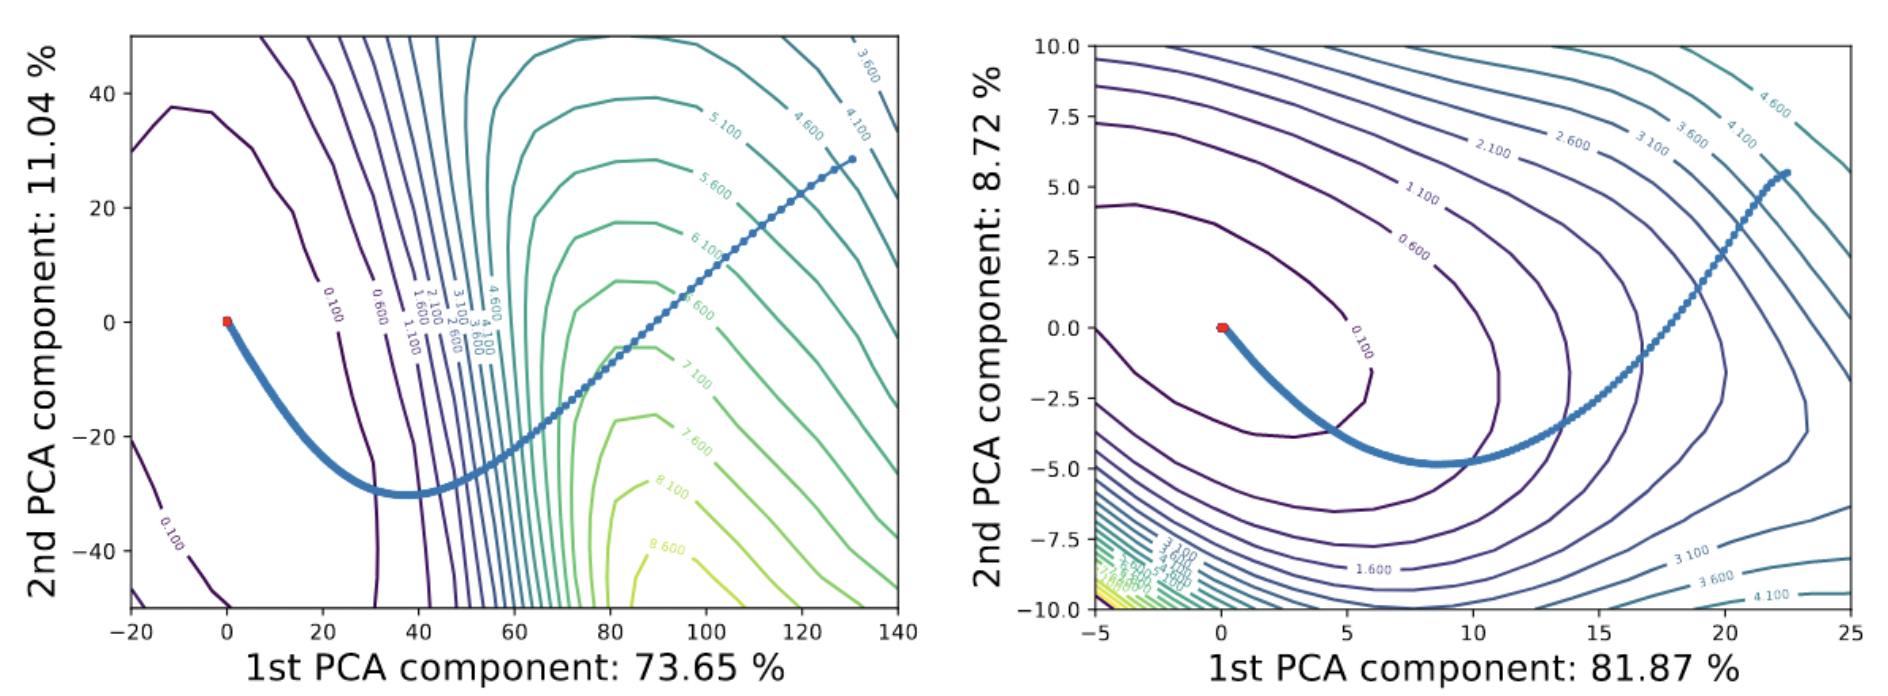
\includegraphics[height=1.07in]{images/traj-plot-SGD.png}
				\\
			\end{array}$
	\end{center}
	\caption{ Plots from the original authors visualizing the model's convergence to a local minimum during gradient descent. } \label{fig:descent_trajectory}
\end{figure}


\bibliographystyle{acmsiggraph}
\nocite{*}
\bibliography{final_project_references}
\end{document}
